\documentclass[10pt]{article}
\usepackage[paper=letterpaper,margin=2cm]{geometry}
\usepackage{amsmath}
\usepackage{amssymb}
\usepackage{amsfonts}
\usepackage{newtxtext, newtxmath}
\usepackage{enumitem}
\usepackage{titling}
\usepackage{graphicx}    %  in the preamble
\usepackage{fancyhdr}
\usepackage{subcaption}
\usepackage[colorlinks=true]{hyperref}

\setlength{\droptitle}{-10em}

\fancyhf{}
\fancyhead[L]{MATH 232: Linear Algebra}
\fancyhead[R]{Steven Wong, 301337727}
\renewcommand\headrulewidth{0pt}
\pagestyle{fancy}

\begin{document}

\noindent\makebox[\textwidth][c]{\Large\bfseries Assignment 4: Machine Learning}
\normalsize
\begin{enumerate}[leftmargin=\labelsep]
    
    \item Using our set of data points I considered hours spent studying per week as input and Math 232 grades as output. The data was fitted
    to a linear function (1) and quadratic function (2). These functions were then fitted with least squares method where $\vec{v} = {(A^{T}A)}^{-1}A^{T}b$.
    The success points were calculated by taking the y-value (Math 232 Grade) and setting it equal to 50 which resulted in 4.56 hours for the linear function
    and 4.45 hours for the quadratic function respectively. Both models are plotted below:

    \begin{figure}[h]
        % Side by side figures 
        \begin{minipage}[c]{0.48\linewidth}
        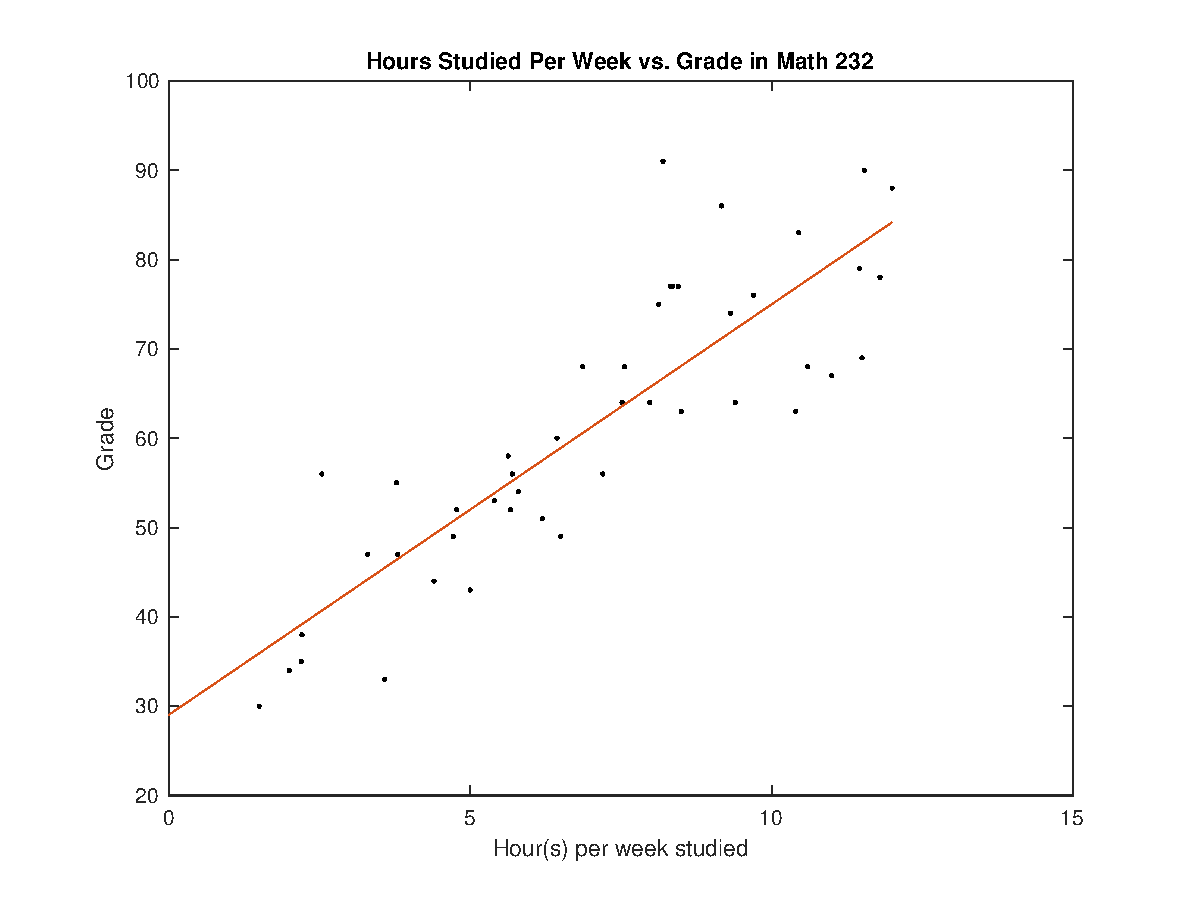
\includegraphics[width=\linewidth]{Linear.eps}
        \end{minipage}
        \hfill
        \begin{minipage}[c]{0.48\linewidth}
        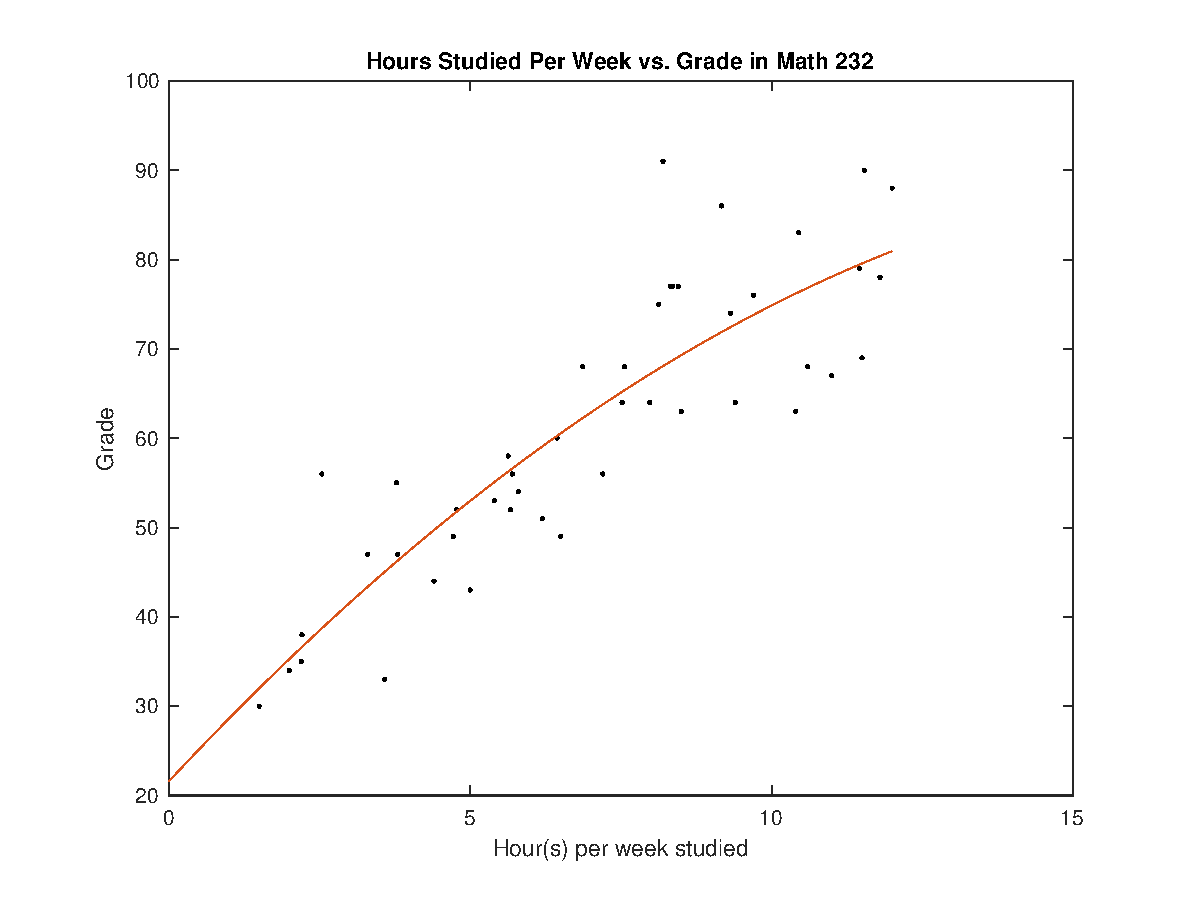
\includegraphics[width=\linewidth]{Quadratic.eps}
        \end{minipage}%
    \end{figure}

    \item Follows similarly from previous material but introduces Math 152 grades as an input variable applied to a linear function (3). The success point was found by setting the z-value (Math 232 grade) equal to 50 percent and solving for the intersection of two planes and projecting it onto the x-y plane.
    This line can be represented by equation (4). The model has been plotted below along with its corresponding line of success in the x-y plane with values above the line representing pass and below representing fail.

    \begin{figure}[h]
        % Side by side figures 
        \begin{minipage}[c]{0.48\linewidth}
        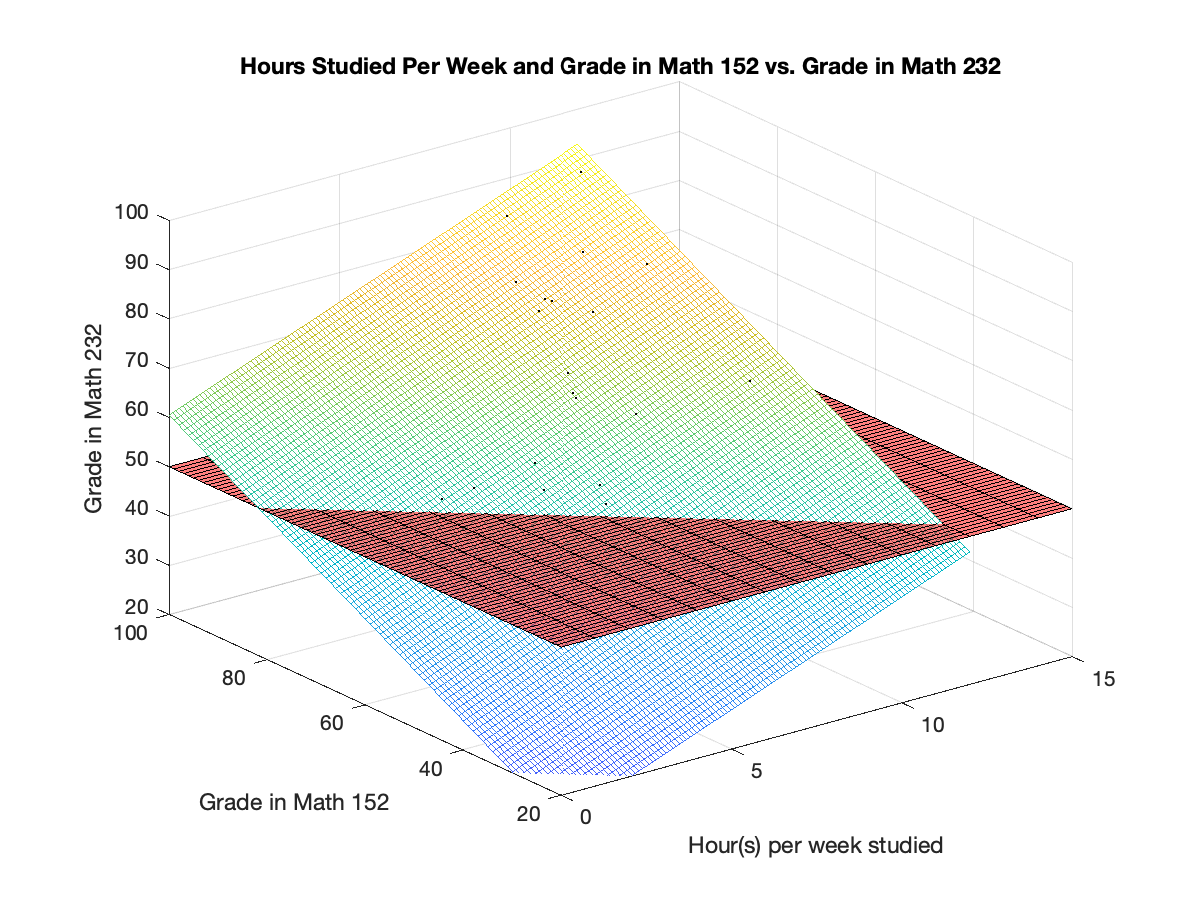
\includegraphics[width=\linewidth]{Multivariate.eps}
        \end{minipage}
        \hfill
        \begin{minipage}[c]{0.48\linewidth}
        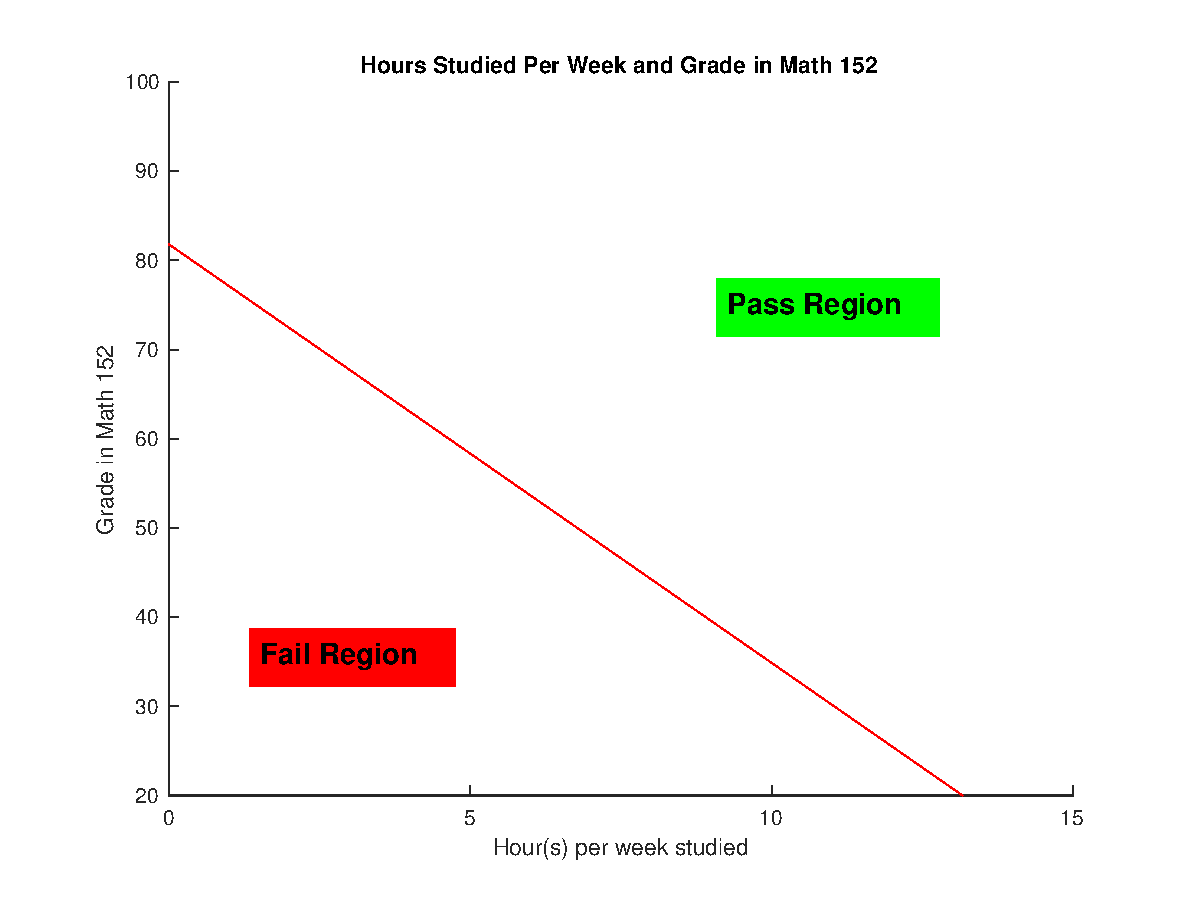
\includegraphics[width=\linewidth]{SuccessLine.eps}
        \end{minipage}%
    \end{figure}

    \begin{equation}
        y = a + bx = \frac{5631}{194} + \frac{409}{89}x
    \end{equation}

    \begin{equation}
        y = a + bx + cx^2 = \frac{8111}{376} + \frac{1396}{193}x - \frac{197}{1034}x^2
    \end{equation}

    \begin{equation}
        z = a + bx + cy = \frac{1967}{706} + \frac{1942}{717}x + \frac{101}{175}y
    \end{equation}

    \begin{equation}
        y = \frac{10553}{129} - \frac{1666}{355}x        
    \end{equation}
    
\end{enumerate}
\end{document}

